% !TeX root = _main.tex
% ROLE 2: muc 5--6, du lieu, phuong phap, phan tich va nguyen nhan.
% Chi sua role cua minh va figures/rX_*. Khong sua tay bang do Python sinh.
% Nguoi ghep bai quan ly _main.tex va _content.tex.
% Cong thuc, bang so chi tiet va bieu mau o role_2_appendix.tex (Phu luc B).
% Macro Role*Supplement cuoi file giu ban nhap mo rong; KHONG duoc goi trong PDF.

\section{Dữ liệu, giả định và phương pháp phân tích}
\label{r2:method}
\subsection{Dữ liệu và giả định}
Nhóm chưa có dữ liệu giao dịch của một cửa hàng thật, nên lượt xe đến trong
báo cáo là \textbf{dữ liệu mô phỏng}. Tuy vậy, quy mô cửa hàng được ước tính từ
số liệu công bố chứ không đặt tùy ý. Hà Nội bán khoảng 110\,000~m$^3$ xăng mỗi
tháng qua 453 cửa hàng~\cite{sct2026}, tức trung bình khoảng 8\,100 lít mỗi
cửa hàng mỗi ngày. Chia lượng xăng này theo số lít mỗi lần đổ, một cửa hàng
đại diện có khoảng 2\,495 lượt xe mỗi ngày. Cách tính chi tiết nằm ở
Phụ lục~\ref{r2:app-params}. Để kiểm tra cách chia lượt xe theo giờ, nhóm dùng
thêm dữ liệu Google Maps của hai cửa hàng tại Hà Nội (Mục~\ref{r2:gmaps}).

Bảng~\ref{r2:assumptions} liệt kê mọi tham số đầu vào và ghi rõ mỗi tham số
lấy từ đâu. Nhãn E là ước tính suy ra từ số liệu công bố, nhãn G là giả định
của nhóm và cần đo lại. Điều đáng chú ý là chỉ ba tham số có nhãn E, còn chín
tham số còn lại đều là G. Nói cách khác, quy mô cửa hàng có căn cứ, nhưng nhịp
xe đến theo giờ và tốc độ phục vụ vẫn là giả định. Nhịp xe đến theo giờ đã được
đối chiếu với Google Maps, còn tốc độ phục vụ chưa có cách kiểm tra.

\begin{table}[htbp]\centering\small
\caption{Tham số đầu vào (E: ước tính từ số liệu công bố; G: giả định cần đo lại)}\label{r2:assumptions}
\begin{tabularx}{\linewidth}{@{}>{\raggedright\arraybackslash}p{42mm}>{\raggedright\arraybackslash}p{54mm}p{8mm}Y@{}}
\toprule
Tham số & Giá trị & Loại & Cách đo lại \\
\midrule
Lượng xăng bán / cửa hàng & 8\,094 lít/ngày & E & Sản lượng bán của cửa hàng \\
Lượt xe / ngày & 2\,495 (xe máy 97,3\%) & E & Đếm hóa đơn điện tử \\
Lượt xe theo giờ $\lambda_t$ & 112--225 xe/giờ & G & Đã đối chiếu Google Maps; giờ trên hóa đơn \\
$E[S]$ xe máy / ô tô & 1,5 / 4,0 phút & G & Bấm giờ tại trụ \\
Độ dao động của $S$ & CV = 0,8 & G & Bấm giờ tại trụ \\
Số vòi / nhân viên & 8 vòi; 6 người mỗi giờ & G & Hỏi cửa hàng \\
Ngưỡng bỏ đi & 20 xe đang chờ & G & Đếm xe bỏ đi \\
Mức giảm $E[S]$ khi trả trước & 20\% & G & Thử tại cửa hàng \\
Chi phí nhân viên & 58\,000 đồng/giờ & E & Bảng lương thật \\
Lãi gộp bán lẻ & 1\,500 đồng/lít & G & Số liệu cửa hàng \\
Chi phí số hóa & 250\,000 đồng/ngày & G & Báo giá \\
Mục tiêu dịch vụ & $E[W_q]\le2$ phút; $P(W_q{>}5)\le5\%$; bỏ đi $\le1\%$ & G & Nhóm đặt \\
\bottomrule
\end{tabularx}
\source{nhóm tổng hợp; căn cứ và nguồn của từng dòng ở Bảng~\ref{r2:assumptions-detail}, Phụ lục~\ref{r2:app-params}}
\end{table}

Trong các giả định, thời gian phục vụ trung bình $E[S]$ ảnh hưởng mạnh nhất,
vì nó quyết định mỗi nhân viên phục vụ được bao nhiêu xe trong một giờ.
Nghiên cứu duy nhất nhóm tìm được có số đo là một trạm ven quốc lộ ở
Indonesia, với 3,89 phút cho một xe máy~\cite{batui}. Trạm này chỉ có 2 làn xe
máy và khoảng 28 xe mỗi giờ, nên con số trên không dùng được cho cửa hàng nội
thành. Với 8 vòi và 225 xe trong giờ cao điểm, mỗi xe
phải được phục vụ dưới 2,13 phút thì hàng chờ mới không dài ra mãi. Nếu mỗi
xe mất 3,89 phút, cửa hàng cần ít nhất 15 nhân viên bơm cùng lúc, quá xa so
với quy mô thực tế. Vì vậy nhóm chọn 1,5 phút cho xe máy, 4 phút cho ô tô, và
coi đây là giá trị cần bấm giờ lại đầu tiên.

Một quan sát khác là ô tô chiếm ít lượt nhưng giữ trụ lâu. Ô tô chỉ chiếm
2,7\% số lượt, nhưng mỗi xe đứng ở trụ lâu gấp 2,7 lần xe máy, nên chiếm
khoảng 7\% tổng thời gian bơm. Tỷ lệ này nhỏ, nên mô hình cho hai loại xe dùng
chung một hàng chờ, với thời gian phục vụ bình quân 1,57 phút.

\subsection{Phương pháp phân tích}
Nhóm dùng hai công cụ bổ sung cho nhau: công thức hàng đợi M/M/c và mô phỏng.
Các ký hiệu $a_i$, $b_i$, $d_i$, $W_q$, $\lambda_t$, $c_t$ và hệ số tải
$\rho$ giữ nguyên định nghĩa ở Mục~\ref{r1:system}. Ba chỉ số chính là thời
gian chờ trung bình $W_q$, tỷ lệ xe chờ quá 5 phút $P(W_q{>}5)$ và tỷ lệ xe
bỏ đi vì hàng quá dài.

Công thức M/M/c cho phép tính nhanh thời gian chờ của từng giờ khi biết
$\lambda_t$, $c_t$ và $E[S]$. Công thức này giả định xe đến ngẫu nhiên theo
phân phối Poisson, thời gian phục vụ theo phân phối mũ, và hàng chờ đã ở trạng
thái ổn định, tức không còn dài thêm hay ngắn đi theo thời gian. Các công thức
lấy theo bài giảng L4~\cite{l4} và được trình bày ở
Phụ lục~\ref{r2:app-formula}. Nhóm dùng công thức này để tìm những giờ thiếu
nhân viên và chọn số kênh sơ bộ.

Mô phỏng dùng để kiểm tra những điều công thức không mô tả được. Chương trình
sinh từng xe đến theo giờ, gán loại xe và thời gian phục vụ, rồi phục vụ theo
thứ tự xe đến trước được bơm trước. Khác với công thức, mô phỏng có hai loại
xe và cho xe bỏ đi khi đã có 20 xe chờ. Số nhân viên trong mô phỏng cũng được
đổi theo từng giờ. Thời gian phục vụ có hệ số biến thiên CV (độ lệch chuẩn
chia cho trung bình) bằng 0,8, tức ít dao động hơn phân phối mũ (CV = 1). Mỗi
phương án được chạy 20 ngày; mã nguồn và nhật ký chạy nằm trong thư mục
\texttt{analysis/}~\cite{analysis}.

\section{Kiểm chứng và phân tích hiện trạng}
\label{r2:diagnosis}
\subsection{Nhu cầu theo giờ}
Hình~\ref{r2:arrivals} cho thấy lượt xe dồn vào buổi chiều tối rõ hơn nhiều so
với buổi sáng. Theo giả định G, cửa hàng có hai đỉnh lúc đi làm và tan tầm.
Giờ đông nhất là 18--19 giờ với 225 xe, gấp đôi giờ vắng nhất. Ba giờ cao
điểm 08--09, 17--18 và 18--19 chỉ chiếm 3/16 thời gian mở cửa nhưng nhận tới
26\% tổng số lượt xe.

\begin{figure}[htbp]\centering
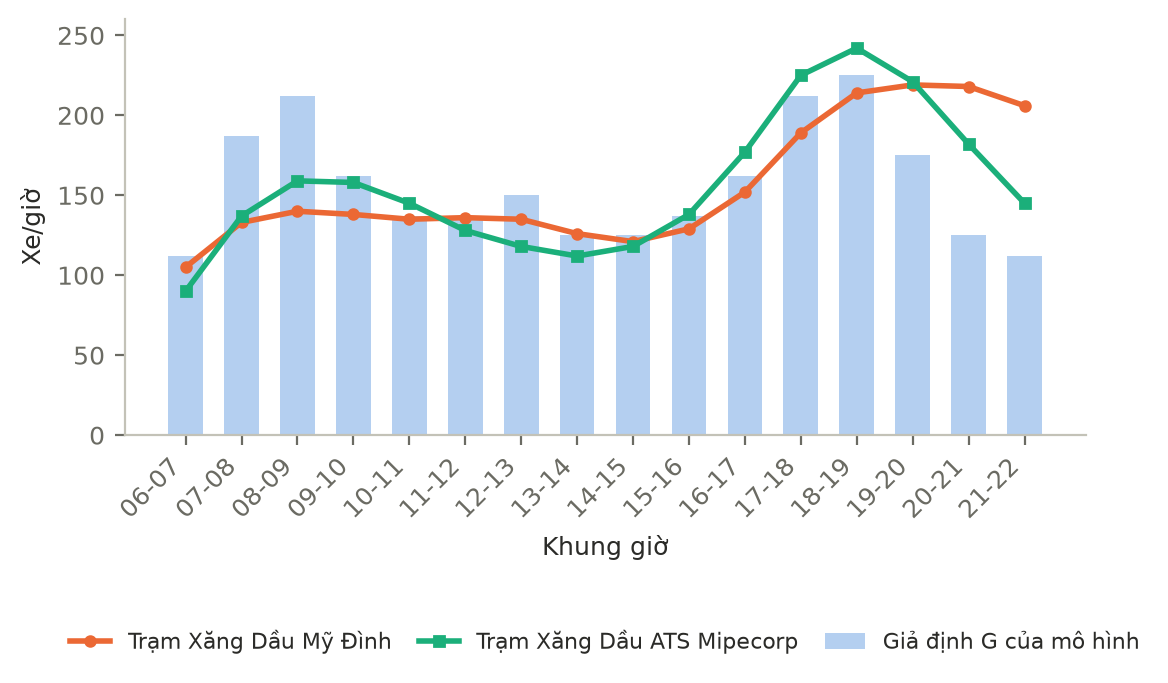
\includegraphics[width=0.78\linewidth]{figures/r2_gmaps.png}
\caption{Lượt xe theo giờ: giả định G của mô hình và phân bố suy từ Google Maps của hai trạm (cùng tổng 2\,495 lượt/ngày)}\label{r2:arrivals}
\source{\texttt{analysis/run\_analysis.py}, \texttt{analysis/gmaps.py}; ảnh Google Maps~\cite{gmaps2026}; số liệu ở Bảng~\ref{r2:gmaps-share}, Phụ lục~\ref{r2:app-tables}}
\end{figure}

Để kiểm tra giả định này, nhóm dùng biểu đồ ``Giờ đông khách'' của Google
Maps. Biểu đồ cho biết mỗi giờ một địa điểm đông đến mức nào so với giờ đông
nhất trong tuần của chính địa điểm đó. Google tính mức này từ vị trí ẩn danh
của người dùng điện thoại, lấy trung bình trong vài tháng gần
nhất~\cite{gmapshelp}. Nhóm chụp biểu đồ đủ 7 ngày của Trạm Xăng Dầu Mỹ Đình
(Lê Quang Đạo) và Trạm Xăng Dầu ATS Mipecorp (Phạm Hùng), đo chiều cao từng cột rồi đổi thành tỷ trọng
theo giờ~\cite{gmaps2026}. Biểu đồ không cho số xe, nên tổng lượt mỗi ngày vẫn
giữ 2\,495. Cách đo nằm ở Phụ lục~\ref{r2:app-plan}.

Dữ liệu của hai trạm chỉ xác nhận đỉnh buổi chiều. Buổi sáng không có đỉnh rõ:
giờ 07--09 chỉ có 133--159 xe, thấp hơn giả định 187--212 xe. Ngược lại, đỉnh
chiều đến muộn hơn và kéo dài hơn. Trạm Mỹ Đình giữ mức 214--219 xe từ 18 đến
21 giờ, và còn 206 xe lúc 21--22 giờ, trong khi giả định chỉ có 112 xe. Trạm
ATS Mipecorp có đỉnh cao hơn giả định, 242 xe lúc 18--19 giờ. Ở cả hai trạm,
giờ đông nhất của hầu hết các ngày là 18--19 giờ. Riêng lúc 20--21 giờ tối thứ
Tư, trạm Mỹ Đình đông gấp 1,5--1,9 lần cùng giờ các ngày khác; nhóm chưa rõ
nguyên nhân.

Sự chênh lệch giữa giờ vắng và giờ đông là gốc của hàng chờ khi lịch nhân viên
cố định. Với 6 nhân viên suốt ngày, công suất cửa hàng không đổi, trong khi
nhu cầu thay đổi khoảng gấp đôi trong ngày. Các phân tích còn lại của báo cáo
vẫn dùng giả định G làm đường cơ sở; phân bố Google Maps được dùng để kiểm tra
lại ở Mục~\ref{r2:gmaps}. Bộ dữ liệu mô phỏng theo giả định G có 50\,144 lượt
xe trong 20 ngày, thời gian phục vụ trung bình 1,568 phút, khớp với tham số đã
đặt (Bảng~\ref{r2:lambda}). Điều này chỉ cho thấy mã chạy đúng thiết kế.

\subsection{Độ tin cậy của công thức M/M/c}
Hình~\ref{r2:validation}a cho thấy công thức và mô phỏng khớp nhau khi tải
vừa phải nhưng lệch xa khi tải gần đầy. Để so sánh công bằng, mô phỏng ở đây
dùng đúng giả định của công thức: một loại xe, thời gian phục vụ phân phối mũ
và không có xe bỏ đi. Với hệ số tải $\rho$ từ 0,73 đến 0,84, hai cách tính
chênh nhau không quá 7,5\%. Ở $\rho=0{,}98$, công thức cho 12,17 phút còn mô
phỏng chỉ cho 7,61 phút, thấp hơn 37,5\%.

\begin{figure}[htbp]\centering
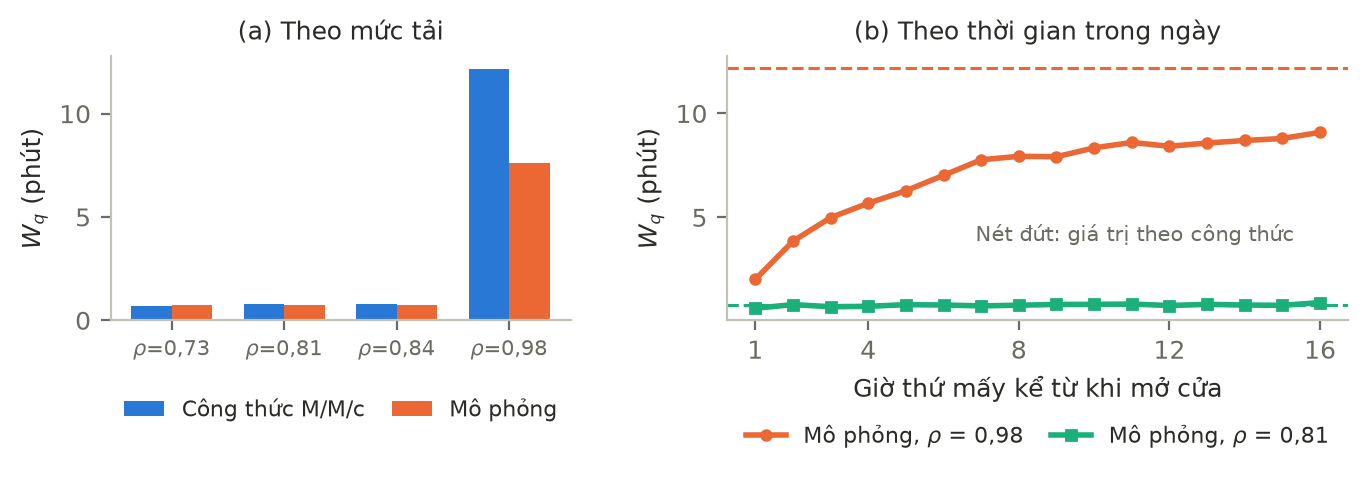
\includegraphics[width=0.86\linewidth]{figures/r2_validation.png}
\caption{So sánh công thức M/M/c với mô phỏng: (a) theo mức tải; (b) thời gian chờ theo giờ kể từ khi mở cửa}\label{r2:validation}
\source{\texttt{analysis/run\_analysis.py}; mô phỏng 40 ngày mỗi cấu hình ở (a), 200 ngày ở (b); số liệu ở Bảng~\ref{r2:validation-table}}
\end{figure}

Chênh lệch này không có nghĩa là mô phỏng sai. Khi tải gần đầy, hàng chờ cần
rất nhiều giờ mới đạt trạng thái ổn định mà công thức giả định. Hình~\ref{r2:validation}b
theo dõi thời gian chờ theo từng giờ kể từ khi mở cửa, khi mỗi ngày bắt đầu
không có xe chờ. Ở $\rho=0{,}81$, thời gian chờ gần bằng giá trị công thức ngay
từ giờ thứ hai. Ở $\rho=0{,}98$, thời gian chờ tăng dần từ 2,0 phút ở giờ đầu
lên 9,1 phút ở giờ thứ 16 mà vẫn chưa chạm mức công thức. Khi nhóm chạy mô
phỏng liên tục 3\,000 giờ, kết quả trung bình của ba lần chạy là 12,32 phút,
rất gần 12,17 phút của công thức. Như vậy, cả hai cách tính đều đúng; chênh
lệch đến từ việc một ngày làm việc quá ngắn để hàng chờ kịp ổn định.

Giờ cao điểm thật chỉ kéo dài một đến hai giờ, nên ở những giờ này công thức
báo thời gian chờ cao hơn thực tế. Vì vậy, nhóm dùng công thức như một phép
kiểm tra thận trọng để tìm giờ thiếu nhân viên, còn mức chờ cụ thể lấy từ mô
phỏng.

\subsection{Điểm nghẽn của lịch hiện tại}
Hình~\ref{r2:asis-load} cho thấy lịch 6 nhân viên cố định thừa người trong
phần lớn thời gian nhưng thiếu người đúng lúc đông nhất. Trong 16 giờ mở cửa,
13 giờ đạt mục tiêu, và từ 09:00 đến 17:00 hệ số tải chỉ từ 0,54 đến 0,71.
Ba giờ còn lại không đạt. Riêng giờ 18--19 có $\rho=0{,}98$, và theo công
thức khoảng 64\% xe phải chờ quá 5 phút.

\begin{figure}[htbp]\centering
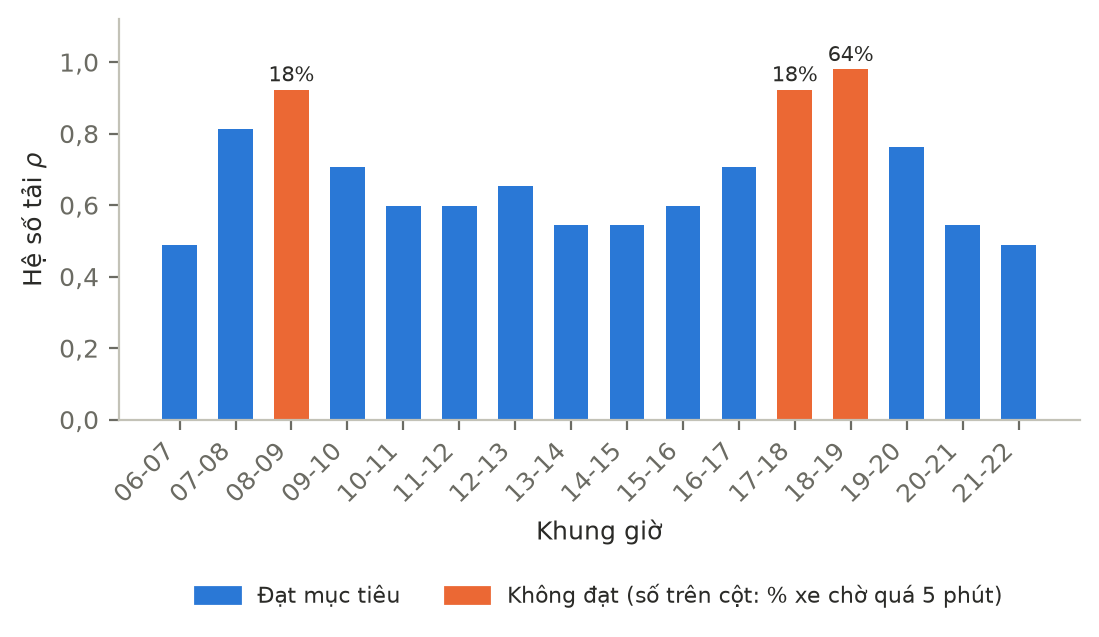
\includegraphics[width=0.7\linewidth]{figures/r2_asis_load.png}
\caption{Hệ số tải theo giờ của lịch hiện tại (6 nhân viên, $E[S]=1{,}57$ phút, công thức M/M/c)}\label{r2:asis-load}
\source{\texttt{analysis/run\_analysis.py}; số liệu đầy đủ ở Bảng~\ref{r2:hourly}, Phụ lục~\ref{r2:app-tables}}
\end{figure}

Vấn đề vì vậy không nằm ở tổng số giờ công mà ở cách chia giờ công trong
ngày. Nếu mỗi giờ chỉ bố trí số nhân viên ít nhất mà vẫn đạt mục tiêu (cách
tính ở Mục~\ref{r3:tobe}), lịch hiện tại thừa 11 giờ công ở các giờ vắng và
thiếu 3 giờ công ở ba giờ cao điểm. Khi $\rho$ vượt khoảng 0,9, gần như không
còn nhân viên rảnh để đỡ lúc xe dồn đến, nên thời gian chờ tăng rất nhanh.

Kết quả mô phỏng cả ngày cho thấy con số trung bình có thể che mất vấn đề.
Tính trên cả ngày, mỗi xe chỉ chờ trung bình 0,64 phút và nhân viên bận 67,9\%
thời gian. Nhưng trong khung 17--19 giờ, 6,2\% xe chờ quá 5 phút và 2,3\% xe
bỏ đi. Mức này thấp hơn nhiều so với con số 64\% của công thức, đúng như phân
tích ở mục trước, nhưng vẫn vượt mục tiêu 5\% và 1\%. Vì vậy chẩn đoán phải
xét theo từng giờ, không theo trung bình ngày.

\subsection{Kiểm tra lại bằng dữ liệu Google Maps}
\label{r2:gmaps}
Khi thay giả định G bằng phân bố của hai trạm, chẩn đoán chính vẫn đúng: lịch
6 người cố định thiếu người vào buổi tối. Bảng~\ref{r2:gmaps-table} chạy lại
mô hình với cùng tổng lượt xe, cùng $E[S]$ và cùng số ngày mô phỏng. Lịch hiện
tại (A0) không đạt mục tiêu ở 4 giờ tại trạm Mỹ Đình (18--22 giờ) và 3 giờ tại
trạm ATS Mipecorp (17--20 giờ). Ở trạm ATS Mipecorp, giờ 18--19 có 16\% xe chờ
quá 5 phút và 1,26\% xe bỏ đi trong ngày, đều cao hơn kết quả theo giả định G.

\begin{table}[htbp]\centering\small
\caption{Lịch hiện tại (A0) và lịch theo giờ (A1) khi lượt xe chia theo giả định G hoặc theo Google Maps}\label{r2:gmaps-table}
\resizebox{\linewidth}{!}{\begin{tabular}{llrrrrrr}
\toprule
\textbf{Phân bố theo giờ} & \textbf{Lịch} & \textbf{Giờ công} & \textbf{Giờ không đạt} & \textbf{$W_q$ (phút)} & \textbf{$P(W_q{>}5)$ (\%)} & \textbf{Bỏ đi (\%)} & \textbf{Giờ tệ nhất: $P(W_q{>}5)$ (\%)} \\
\midrule
Giả định G & A0 & 96 & 3 & 0{,}64 & 1{,}68 & 0{,}49 & 18-19: 8{,}0 \\
Giả định G & A1 & 88 & 0 & 0{,}45 & 0{,}33 & 0{,}04 & 21-22: 1{,}4 \\
Mỹ Đình & A0 & 96 & 4 & 0{,}62 & 1{,}33 & 0{,}35 & 19-20: 5{,}9 \\
Mỹ Đình & A1 & 88 & 3 & 1{,}11 & 8{,}42 & 2{,}92 & 21-22: 89{,}4 \\
Mỹ Đình & A1 lập lại & 87 & 0 & 0{,}48 & 0{,}43 & 0{,}04 & 16-17: 2{,}6 \\
ATS Mipecorp & A0 & 96 & 3 & 0{,}76 & 2{,}64 & 1{,}26 & 18-19: 16{,}0 \\
ATS Mipecorp & A1 & 88 & 4 & 0{,}81 & 3{,}36 & 0{,}66 & 21-22: 25{,}7 \\
ATS Mipecorp & A1 lập lại & 85 & 0 & 0{,}57 & 0{,}56 & 0{,}07 & 14-15: 2{,}3 \\
\bottomrule
\end{tabular}
}
\source{\texttt{tables/tab\_gmaps.tex}; mô phỏng 20 ngày, $E[S]$ hiện tại; ``giờ không đạt'' tính bằng M/M/c; ``A1 lập lại'' là lịch A1 tính lại theo phân bố của từng trạm}
\end{table}

Ngược lại, lịch A1 lập theo giả định G không dùng được cho hai trạm này. Lịch
A1 xếp nhiều người lúc 07--09 giờ và bớt người sau 20 giờ, đúng lúc hai trạm
còn đông. Ở trạm Mỹ Đình, giờ 21--22 chỉ có 4 người cho 206 xe, tức
$\rho=1{,}35$, nên 89\% xe chờ quá 5 phút và 2,9\% xe bỏ đi trong ngày. Kết quả
này còn tệ hơn lịch cố định. Khi lập lại lịch theo đúng phân bố của từng trạm,
A1 đạt mục tiêu ở mọi giờ với 87 và 85 giờ công, gần bằng 88 giờ công của A1
ban đầu.

Như vậy, cách lập lịch theo giờ vẫn đúng, nhưng lịch cụ thể phải tính riêng
cho từng cửa hàng từ dữ liệu của chính cửa hàng đó. Các con số ở
Mục~\ref{r3:tobe} dựa trên giả định G, nên chỉ nên đọc như kết quả của một
cửa hàng minh họa.

\subsection{Nguyên nhân và giới hạn của chẩn đoán}
Kết quả trên chỉ ra hai nguyên nhân có thể kiểm tra riêng. Nguyên nhân thứ
nhất là số nhân viên giữ cố định trong khi lượt xe thay đổi theo giờ. Phương
án A1 ở Mục~\ref{r3:tobe} kiểm tra nguyên nhân này mà không đổi thời gian phục
vụ. Nguyên nhân thứ hai là khách trả tiền ngay tại trụ, làm xe đứng lâu hơn.
Phương án A2 kiểm tra giả định rằng trả trước giúp rút ngắn thời gian này
20\%; con số 20\% chưa được chứng minh.

Mô hình chưa xét các nguyên nhân khác như lối ra vào chật, vòi hỏng, hết
một loại xăng hay tốc độ làm việc khác nhau giữa các nhân viên. Cần kiểm tra
chúng bằng số liệu thật trước khi kết luận.

Dữ liệu Google Maps cũng có giới hạn. Biểu đồ chỉ cho độ đông tương đối chứ
không cho số xe, và có thể tính cả người ghé cửa hàng tiện lợi hay đi ngang
qua. Hai trạm đều mở 24 giờ, trong khi mô hình chỉ xét 06--22 giờ, khung giờ
chiếm 79\% và 88\% độ đông cả ngày của hai trạm. Quan trọng hơn, Google Maps
không cho biết thời gian phục vụ $E[S]$. Đây vẫn là giả định ảnh hưởng mạnh
nhất mà nhóm chưa kiểm chứng được.

\newcommand{\RoleTwoSupplement}{%
\section{Mô hình mở rộng: định vị rời rạc và dự báo nhu cầu}
\label{r2:extension}
\subsection{Chọn 2 trong 5 điểm mở cửa hàng mới}
\label{r2:location}
\textbf{Bài toán.} Doanh nghiệp có ngân sách mở $k=2$ cửa hàng mới và đã khảo
sát 5 vị trí ứng viên $J$ trên các trục chính; nhu cầu đến từ 8 quận $I$.
Bài toán định vị phân bố được rời rạc hóa bằng hai tập này. Dân số lấy theo
Tổng điều tra 2019~\cite{census2019}; nhu cầu mà một cửa hàng mới có thể thu
hút ở vùng $i$ là
\begin{equation}
h_i=\text{dân số}_i\times0{,}695\ \tfrac{\text{xe}}{\text{người}}\times0{,}2\
\tfrac{\text{lượt}}{\text{xe}\cdot\text{ngày}}\times2\%\ \text{(thị phần)},
\end{equation}
với 0,695 = 5,6 triệu xe máy xăng (2025)~\cite{vnex2025} / 8,05 triệu dân (2019) (E), 0,2 lượt/ngày = đổ 2,5 lít
mỗi 5 ngày (E), thị phần 2\% (G). Thời gian đi lại $t_{ij}$ (phút) tính từ tọa
độ xấp xỉ: khoảng cách đường chim bay $\times1{,}35$ (hệ số đường vòng), tốc
độ 20~km/giờ giờ cao điểm, cộng 2 phút ra/vào. Ngưỡng tiếp cận $R=15$ phút.
Năng lực một cửa hàng 8 vòi là $Q_j=2\,889$ lượt/ngày: giờ cao điểm (9\% lượt
ngày) tối đa 260 xe/giờ để vẫn đạt $\rho\le0{,}85$, $W_q\le2$ phút. Chi phí cố
định $f_j$ (thuê đất, khấu hao, quản lý) là 120, 150, 80, 95, 75 triệu đồng/tháng
cho J1--J5 (G). Mỗi lượt đóng góp $3{,}24\times1\,500-2\,165\approx2\,700$ đồng
(lãi gộp trừ lương nhân viên theo lượt).

\textbf{Mô hình.} $a_{ij}=1$ nếu $t_{ij}\le R$ (mã hóa nhị phân); vùng $i$ được
phủ khi tồn tại $j$ có $a_{ij}=1$ và $y_j=1$. Quyết định mở điểm được tích hợp
với phân bổ nhu cầu, chỉ giao cho điểm đã mở và không vượt năng lực:
\begin{align}
\text{(a)}\ \max\ \textstyle\sum_i h_i z_i \quad\text{hoặc}\quad
\text{(b)}\ \max\ 30\cdot2\,700\textstyle\sum_i h_i z_i/10^6-\sum_j f_j y_j \label{r2:mclp}\\
\text{với}\ \textstyle\sum_j y_j=2,\ x_{ij}\le a_{ij}y_j,\ \sum_j x_{ij}=z_i\le1,\
\sum_i h_i x_{ij}\le Q_j y_j,\ x,y,z\in\{0,1\}. \nonumber
\end{align}
Mục tiêu (a) là phục vụ được nhiều người nhất; mục tiêu (b) là lợi nhuận
(triệu đồng/tháng). Với $\binom52=10$ tổ hợp, nhóm liệt kê toàn bộ cách giao
vùng nên nghiệm là tối ưu chính xác.
\exttable{tab_ext_cover_matrix.tex}{Dân số, nhu cầu $h_i$ và thời gian đi lại $t_{ij}$ (phút); $^{\bullet}$ đánh dấu $a_{ij}=1$ ($t_{ij}\le15$ phút)}{r2:cover}
\exttable{tab_ext_location.tex}{Mười tổ hợp 2/5 điểm, xếp theo mục tiêu (a); lợi nhuận theo mục tiêu (b)}{r2:loc-result}
\begin{figure}[htbp]\centering
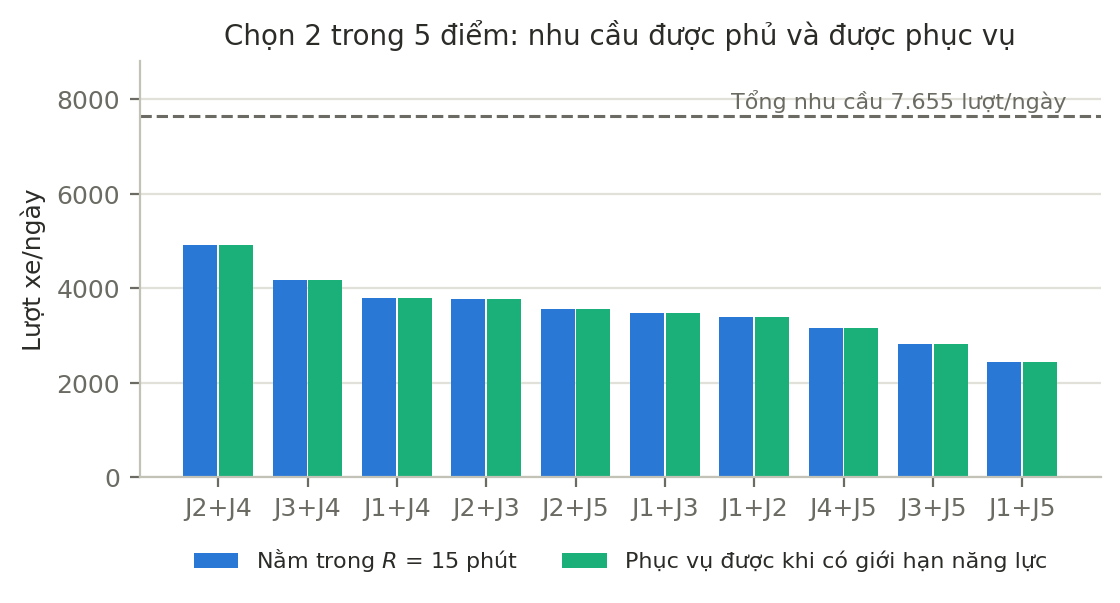
\includegraphics[width=0.9\linewidth]{figures/r2_location.png}
\caption{Nhu cầu nằm trong ngưỡng $R$ và nhu cầu phục vụ được của mười tổ hợp.}
\label{r2:loc-fig}
\source{\texttt{analysis/extension\_analysis.py}; dân số 2019, các tham số còn lại là ước tính/giả định}
\end{figure}

\textbf{Hai mục tiêu cho hai câu trả lời.} Theo mục tiêu (a), \textbf{J2 Đống Đa +
J4 Hoàng Mai} phục vụ 4\,916 lượt/ngày (64,2\% nhu cầu); J2 nhận Cầu Giấy, Đống
Đa, Thanh Xuân (2\,664 lượt/ngày, $\rho_{\max}=0{,}78$). Theo mục tiêu (b),
\textbf{J3 Hà Đông + J4 Hoàng Mai} lãi 163,2 triệu đồng/tháng so với 153,2 triệu
của J2 + J4, dù chỉ phục vụ 54,5\% nhu cầu: J2 nằm ở vùng giá thuê cao
(150 triệu đồng/tháng) và phải gánh tải gần năng lực. Một doanh nghiệp tư nhân
chịu áp lực chiết khấu thấp sẽ chọn (b); nếu mục tiêu là độ phủ dịch vụ (ví
dụ cam kết với đầu mối về sản lượng), (a) phù hợp hơn.

\exttable{tab_ext_location_sens.tex}{Độ nhạy của quyết định định vị}{r2:loc-sens}
\textbf{Độ bền.} J3 + J4 là tổ hợp lãi nhất ở 5/6 tình huống: $R=15$ hoặc 20
phút, nhu cầu giảm 20\% (KB-A), tăng 20\% (KB-B) và cửa hàng chỉ có 6 vòi; khi
nhu cầu tăng 20\%, J3 + J4 còn trở thành phương án phục vụ nhiều nhất vì J2 bị
giới hạn năng lực. Ngược lại, lợi nhuận của J2 + J4 giảm còn 73,6 triệu khi
nhu cầu giảm 20\% và còn 18,9 triệu nếu chỉ có 6 vòi. Chỉ khi $R=12$ phút (khách
rất ngại đi xa) thì tối ưu lợi nhuận chuyển sang J4 + J5.

\exttable{tab_ext_location_econ.tex}{Độ nhạy lợi nhuận BT2 theo lãi gộp (G) và chi phí cố định $f_j$ (G); số lượt phục vụ của từng tổ hợp giữ nguyên}{r2:loc-econ}
\textbf{Điều kiện kinh tế.} Hai tham số quyết định mục tiêu (b) đều là giả định:
lãi gộp 1\,500 đồng/lít và chi phí cố định $f_j$. Bảng~\ref{r2:loc-econ} tính
lại lợi nhuận khi thay đổi hai tham số này. Số lượt phục vụ không phụ thuộc vào
chúng nên giữ nguyên. Lãi gộp hòa vốn là 1\,098 đồng/lít với J3 + J4 và 1\,180
đồng/lít với J2 + J4. Ở mức 700 đồng/lít, ngưỡng bù chi phí mà~\cite{chietkhau}
nêu, mỗi lượt chỉ đóng góp 106 đồng và không tổ hợp nào có lãi. Ở mức 1\,000
đồng/lít cũng vậy. Ngay cả khi có lãi, lựa chọn giữa J2 và J3 vẫn đảo chiều:
J2 + J4 lãi hơn khi lãi gộp đạt 2\,000 đồng/lít hoặc khi $f_j$ giảm 30\%,
còn J3 + J4 lãi hơn khi $f_j$ tăng 30\%. Kết luận BT2 vì vậy có ba phần.
(i) \textbf{Chỉ mở thêm cửa hàng khi lãi gộp thực tế đạt trên khoảng 1\,100
đồng/lít.} (ii) \textbf{J4 Hoàng Mai} có mặt trong mọi phương án lãi nhất (Bảng~\ref{r2:loc-sens} và~\ref{r2:loc-econ}).
(iii) Điểm thứ hai là J3 Hà Đông nếu ưu tiên lợi nhuận ở mức cơ sở, hoặc J2
Đống Đa nếu ưu tiên độ phủ hay giá thuê thấp hơn giả định. Cần lấy lãi gộp
thật và báo giá thuê của từng điểm trước khi quyết định.
\todo{2}{Thay tọa độ xấp xỉ bằng địa chỉ ứng viên thật và thời gian đi lại từ
bản đồ số; kiểm tra lại số cửa hàng đối thủ trong bán kính $R$ để hiệu chỉnh thị phần 2\%.}

\subsection{Dự báo lượt xe ngày tới bằng học máy}
\label{r2:forecast}
Lịch theo giờ (BT1) chỉ tốt khi biết trước $\lambda_t$. Nhu cầu xăng có các
biến động \emph{biết trước được}: giá điều chỉnh có hiệu lực lúc 15 giờ, phần
lớn vào thứ Năm (các kỳ 22/10, 29/10, 5/11, 12/11/2026), đôi khi có kỳ bổ sung
giữa tuần (31/10, 3/11/2026)~\cite{moit2026,moit2026b}. Khi giá tăng, khách đổ
trước 15 giờ; khi giá giảm, khách chờ sau 15 giờ. Các biến động khác là tuần trước
Tết và kỳ nghỉ Tết, và tín hiệu căng thẳng nguồn cung. Nhóm dựng lịch sử 2 năm
(25/11/2024--22/11/2026) với \emph{lịch sự kiện thật}: Tết Ất Tỵ 29/1/2025, Tết
Bính Ngọ 17/2/2026, đợt cửa hàng đóng cửa giữa 2025 và đợt 17 cửa hàng tạm
dừng bán đầu tháng 3/2026~\cite{vtc2026}; biên độ điều chỉnh giá theo tuần lấy
quanh mức của các kỳ gần đây (E10RON95-III giảm 2\,075 đồng/lít ngày 5/11 và
1\,311 đồng/lít ngày 12/11/2026~\cite{moit2026b,moit2026}). Lượt xe
trong lịch sử là mô phỏng. Mô hình học máy là hồi quy Poisson (GLM, ước lượng IRLS):
\begin{multline}
\log\lambda_{d,h}=\beta_h+\gamma_{\text{thứ}(d)}+\delta_1\sin\tfrac{2\pi d}{364}+\delta_2\cos\tfrac{2\pi d}{364}
+\tau_1 T^{\text{trước}}_d+\tau_2 T^{\text{nghỉ}}_d\\
+\pi_1\Delta p_d\mathbf 1_{h<15}+\pi_2\Delta p_d\mathbf 1_{h\ge15}+\pi_3\Delta p_{d-1}+\eta s_{d-1}+\kappa\ell_{d-1},
\end{multline}
với $\Delta p_d$ là mức điều chỉnh dự kiến (nghìn đồng/lít, tính được trước từ
giá thế giới), $s_{d-1}$ là tín hiệu nguồn cung hôm trước, $\ell_{d-1}$ là log tỷ
số lượt hôm trước so với trung bình 28 ngày. Học trên 23/12/2024--4/1/2026,
kiểm tra trên 84 ngày 5/1--29/3/2026 (có Tết và đợt tháng 3).
\exttable{tab_ext_ml_acc.tex}{Độ chính xác dự báo trên 84 ngày kiểm tra; ``ngày sự kiện'' là 25 ngày có Tết, điều chỉnh giá $\ge$1\,000 đồng/lít hoặc căng thẳng nguồn cung}{r2:ml-acc}
\begin{figure}[htbp]\centering
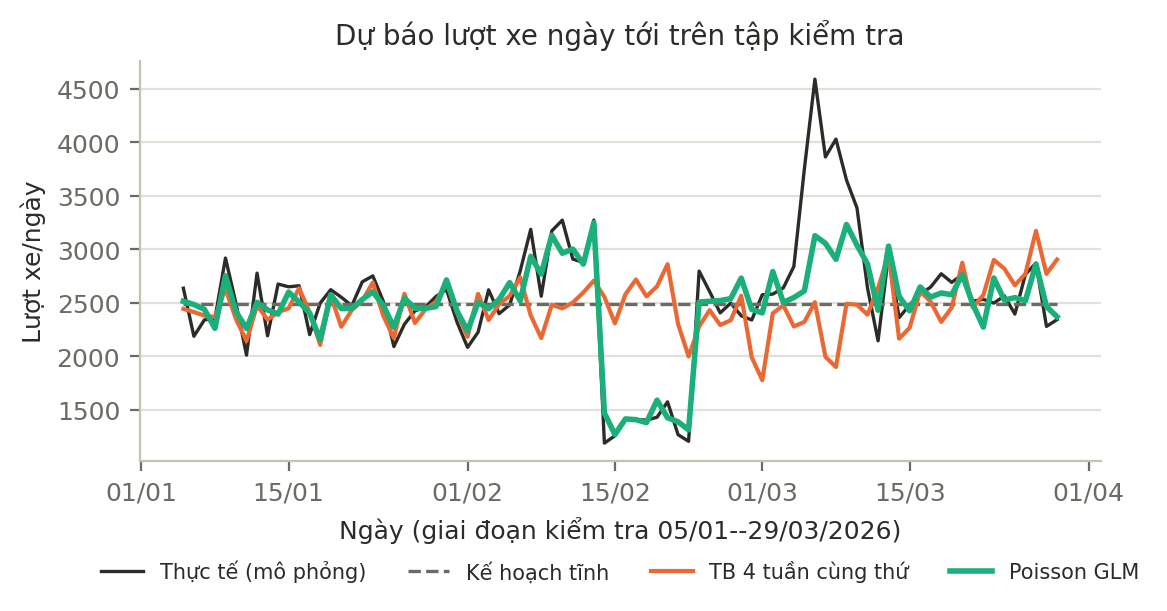
\includegraphics[width=0.9\linewidth]{figures/r2_forecast.png}
\caption{Dự báo tổng lượt xe/ngày trên tập kiểm tra.}\label{r2:ml-fig}
\source{\texttt{analysis/extension\_analysis.py}; lượt xe mô phỏng, lịch sự kiện theo thực tế}
\end{figure}
GLM giảm MAPE tổng ngày từ 18,33\% (kế hoạch tĩnh) và 19,63\% (trung bình 4 tuần
cùng thứ) xuống 7,25\%; trên 25 ngày sự kiện, từ khoảng 46\% xuống 10,44\%.
Trung bình 4 tuần thậm chí kém kế hoạch tĩnh vì nó ``nhớ'' Tết và đợt tháng 3
sang các tuần sau (Hình~\ref{r2:ml-fig}).

\textbf{Cần đọc kết quả này đúng mức.} Lịch sử lượt xe được mô phỏng với các
hiệu ứng do nhóm tự đặt: tuần trước Tết $\times1{,}20$, kỳ nghỉ Tết
$\times0{,}55$, mỗi nghìn đồng/lít tăng giá làm lượt xe trước 15 giờ tăng 25\%.
Mô hình ước lượng lại được gần đúng các giá trị này: $e^{0{,}167}=1{,}18$,
$e^{-0{,}540}=0{,}58$ và $e^{0{,}249}=1{,}28$. Điều đó chỉ cho thấy cách xây
biến và ước lượng là đúng: mô hình tìm lại được cấu trúc đã cài vào dữ liệu.
Đây \emph{không} phải bằng chứng về hành vi của khách thật. Cũng vì dữ liệu và
mô hình có cùng cấu trúc, MAPE 7,25\% là giới hạn trên lạc quan. Độ chính xác
thật chỉ biết được khi huấn luyện trên hóa đơn điện tử.
Giá trị vận hành của dự báo được đánh giá ở Mục~\ref{r3:ml-staff}.
\todo{2}{Huấn luyện lại trên dữ liệu hóa đơn điện tử thật; giữ cách chia theo
thời gian (không trộn ngẫu nhiên) và báo cáo MAPE theo tháng.}

}
